\documentclass[12pt]{article}
 
\usepackage[utf8x]{inputenc}
\usepackage[brazilian]{babel}
\usepackage{fontenc}
\usepackage{graphicx} 
\usepackage{listings}
\usepackage{xcolor}
\usepackage{indentfirst}
\usepackage{rotating}
\usepackage{pdflscape}
%\usepackage[defaultmono]{droidmono}
\usepackage[bottom=3cm,top=3cm,left=3cm,right=3cm]{geometry}

%\renewcommand*\rmdefault{droidmono}


\lstset{
    language=java,
    keywordstyle=\bfseries\ttfamily\color[rgb]{0,0,1},
    identifierstyle=\ttfamily,
    commentstyle=\color[rgb]{0.133,0.545,0.133},
    stringstyle=\ttfamily\color[rgb]{0.627,0.126,0.941},
    showstringspaces=false,
    basicstyle=\small,
    tabsize=2,
    breaklines=true,
    frame=single
}

\title{Programação Orientada a Objetos \\ Trem vol. 1}

\author{David Sena Oliveira}

\date{Quixadá, Outubro de 2014}

\renewcommand{\tt}[1]{\lstinline|#1|}
\renewcommand{\bf}[1]{\textbf{#1}}
\newcommand{\code}[1]{\emph{#1}}
\newcommand{\n}{\lstinline|\n|}

\begin{document}

\begin{figure}
\centering

\includegraphics[width=0.4\linewidth]{ufc}
\label{fig:ufc}
\end{figure}

\maketitle

\section{Descrição}

O \bf{Trem de Ferro} é um dos transportes públicos mais comuns na Europa. Um trem é composto por uma locomotiva e uma quantidade variáveis de vagões, chamada de composição. Uma locomotiva possui um limite máximo de vagões que pode locomover e é responsável por movimentar a composição. Cada vagão pode transportar uma quantidade máxima de passageiros. Assim, vagões são ocupados gradativamente, onde um passageiro só pode ir para o segundo vagão quando o primeiro já estiver totalmente ocupado. O objetivo desse programa é permitir que passageiros possam ser embarcados, desembarcados, buscados e listados nos vagões do trem.


\section{Diagrama}
O diagrama da Figura \ref{fig:diagrama} apresenta as classes a serem implementadas.
\begin{landscape}
%\begin{sidewaysfigure}
\begin{figure}
\centering
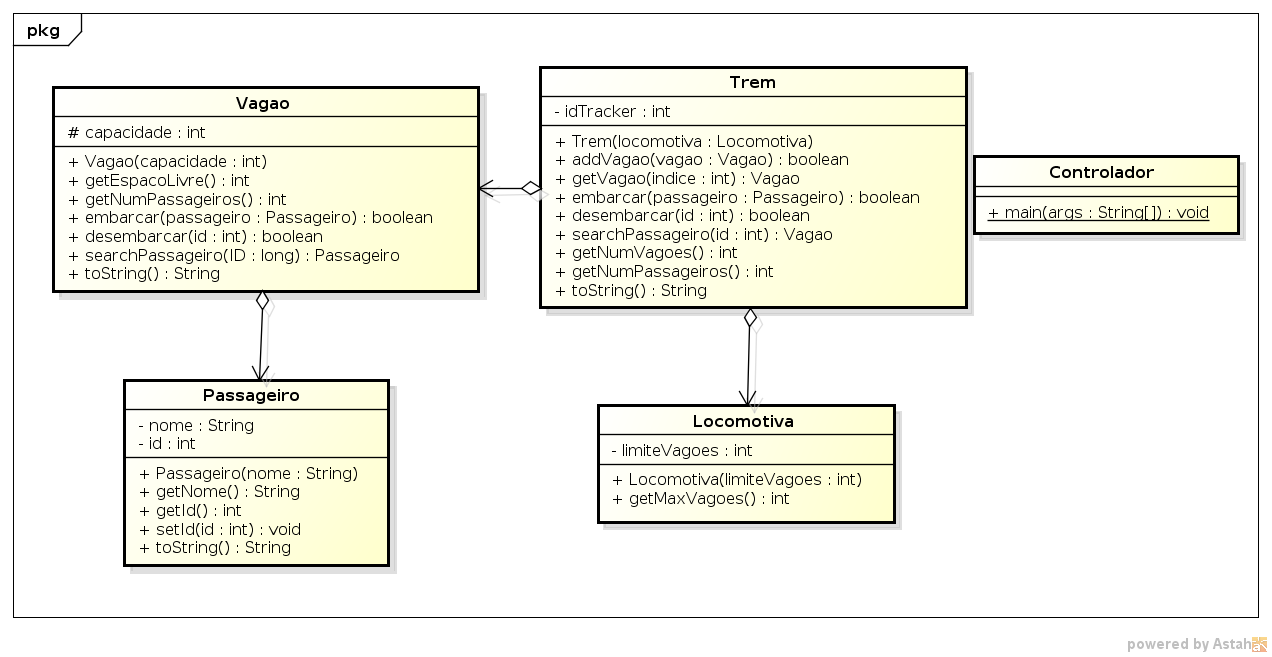
\includegraphics[width=1\linewidth]{./diagrama}
\caption{Diagrama de Classes}
\label{fig:diagrama}
\end{figure}
%\end{sidewaysfigure}
\end{landscape}

\section{Métodos}
A maioria dos métodos, principalmente os \bf{get} e \bf{set} são de implementação trivial. Os métodos não
triviais estão descritos abaixo.

\subsection{Passageiro}
	\begin{itemize}
		\item Construtor recebe apenas o nome do passageiro. O \tt{id} deve ser iniciado com 0.
		\item Método \tt{toString()} deve ser sobrescrito para o seguinte:
		\begin{lstlisting}
public String toString() {
    return id + ":" + nome;
}
		\end{lstlisting} 
	\end{itemize}

\subsection{Locomotiva}
	\begin{itemize}
	\item A Locomotiva é trivial.
	\end{itemize}
	
\subsection{Vagão}
\begin{itemize}
\item Método \tt{int getEspacoLivre()} calcula o espaço livre no vagão, dado pela \bf{capacidade} - numero de passageiros.

\item Método \tt{boolean embarcar(Passageiro passageiro)}  adiciona um passageiro no vagão observando o espaço livre disponível. Ele retorna verdadeiro se operação foi concluída com sucesso ou falso caso contrário;
\item Método \tt{boolean desembarcar(int id)} desembarca o passageiro do vagão que possui o id igual ao passado como parâmetro. Ele retorna verdadeiro se a operação foi concluída com sucesso ou falso caso contrario;
\item Método \tt{Passageiro searchPassageiro(int id)} retorna o passageiro do vagão que possui o id igual ao passado como parâmetro. Caso ele não encontre o passageiro, ele retorna \tt{null};
\item Método \tt{String toString()}

Retorna uma String contendo a descrição do vagão. Deve iniciar com um [.
Depois colocar o nome de cada um dos passageiros na ordem em que eles foram embarcados separando por espaço. Coloque \_ para cada cadeira livre.
Exemplo para vagão com capacidade 5 e duas pessoas embarcadas.

\verb|[ 1:Carlos 2:Mario _ _ _ ]|

\end{itemize}

\subsection{Trem}
\begin{itemize}
\item Método \tt{void addVagao(Vagao vagao)} que adiciona um vagão ao trem observando o número máximo de vagões suportado pela locomotiva;
\item Método \tt{boolean embarcar(Passageiro passageiro)} que embarca um passageiro no trem no primeiro vagão com espaço livre disponível. Ele chama os métodos embarcar
do vagão, delegando as verificações de espaço livre ao vagão. Encontrando um vagão disponível, ele usa o método \tt{passageiro.setId(int id)} configurar o id do passageiro. Cada novo passageiro que embarca deve receber
um novo id. Use o atributo idTracker para guardar manter o controle do próximo id. Ele retorna verdadeiro se o passageiro embarcou ou falso caso contrário;
\item Método \tt{boolean desembarcar(int id)} faz o desembarque do passageiro no vagão onde ele se encontra. Ele retorna verdadeiro se o passageiro desembarcou ou falso caso contrário;
\item Método \tt{Vagao searchPassageiro(int id)} procura o passageiro pelo id percorrendo todos os vagões até o encontrar. Caso encontre, retorna a referência ao vagao que ele está, caso ele não encontre o passageiro, retorna null;
\item Sobrescreva o método \tt{String toString()} para gerar uma String com iniciando com "Trem \{", chamando o método \tt{toString()} de cada vagão e finalizando com um "\}". A saída do comando resulta em algo como 

\verb|Trem{[ 4:Davi ][ 2:Bruno 3:Carlos _ _ ]}|

\end{itemize}

\subsection{Controlador}
O controlador é brinde. Dado, o controlador abaixo, 
a saída gerada deve ser algo como:

\begin{lstlisting}[label=saida, caption=Saida Esperada, float=ht]
Trem: {[ 1:A ][ 2:B 3:C ]}
Trem: {[ _ ][ 2:B 3:C ]}
Trem: {[ 4:D ][ 2:B 3:C ]}
\end{lstlisting}

\pagebreak
\noindent
\bf{Classe Controlador}
\lstinputlisting{controlador.java}

\end{document}
